
\section{Effective mass measurements}


\subsubsection{Basic LK formula fitting}

A series of field sweeps were taken with $H$ at \unit[12]{\degree}, \unit[28]{\degree} and \unit[46]{\degree} from $[001]$ in the $[110]$ direction. These were performed at a variety of temperatures from base ($\approx\unit[0.3]{K}$) to above \unit[2]{K}. \Fig~\ref{Fig:3:ExampleLKFits} shows the Fourier amplitude of various peaks as a function of temperature along with fits to equation~\ref{Eqn:2:TempTermOscillationAmp}. The field range for the FFT was was necessarily large enough that individual peaks did not overlap and also could be observed across a reasonable range of temperatures but also small enough so that the $B$ dependent Dingle factor did not play too large a role and so an average $B$ field can be assumed.

\begin{figure}[h!]
    \begin{center}
        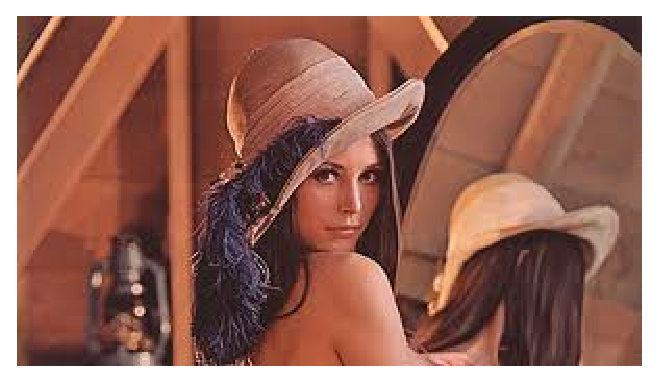
\includegraphics[scale=0.7]{Misc/TODO}
        \caption{}
        \label{Fig:3:SimpleLKFits}
    \end{center}
\end{figure}

\subsubsection{Retrofitting ansatz LK formulae}

The measurements presented in the previous section were further refined using the the ansatz LK formulae as described in section~\ref{Sec:2:LKRetrofitting}. \Fig~\ref{Fig:3:RetrofittedLKFits}
%%
\begin{figure}[h!]
    \begin{center}
        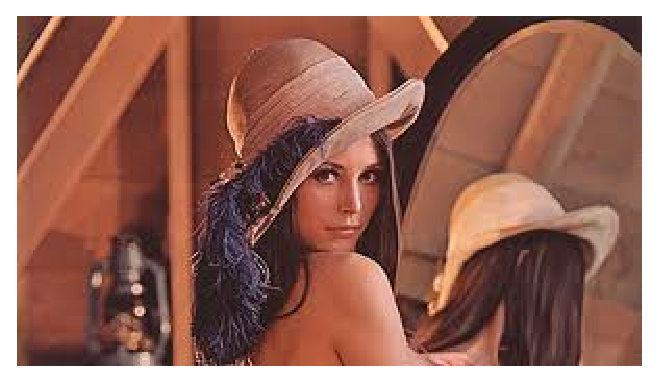
\includegraphics[scale=0.7]{Misc/TODO}
        \caption{}
        \label{Fig:3:RetrofittedLKFits}
    \end{center}
\end{figure}

\subsubsection{`Microfitting' the LK formula}

A second attempt at refining the LK fits was performed by applying the microfit technique desribed in section~\ref{Sec:2:LKMicrofitting}

\subsection{Effective mass results}

Table~\ref{Table:3:EffectiveMasses} lists the results of the effective mass investigations.
%%
\medskip
%%TODO
\begin{center}
    \begin{tabular}[h!]{llr}
\toprule
Band    & \multicolumn{2}{l}{Energy Shift (\unit{Ry})} \\
\midrule
1       &       & -0.0083      \\
2       & Wide  & 0.0          \\
        & Narrow & -0.0038     \\
3       &       & 0.0043       \\
4       &       & 0.0050        \\
\bottomrule
    \label{Table:3:EnergyShifts}
    \end{tabular}
\end{center}

